%!TEX root = ../thesis.tex
\renewcommand\thechapter{A}
\chapter{Appendix A: Time division}
\label{AppendixA}

This Appendix contains two types of time division that represent the content of the \Quote{Piano di Lavoro}: a table with the hours spent per task and a Gantt Diagram.
For each of these there are two iterations, the \Quote{estimated} one and the \Quote{final} one, calculated before and after the internship.

\section{Estimated time spent per task}
	\begin{tabularx}{\textwidth}{c|X}
		\centering\textbf{Hours spent} & \multicolumn{1}{c}{\textbf{Task}}\\\hline
		\textbf{70}&\textbf{Learning the technologies}\\\hline
		\textbf{20}&\textbf{Requirements analysis}\\\hline
		\textbf{40}&\textbf{Setting up the environment}\\\hline
		\textbf{50}&\textbf{Configuration of the services}\\\hline
		\textbf{60}&\textbf{Integration}\\\hline
		\textbf{100}&\textbf{Test}\\\hline
		\textbf{20}&\textbf{Writing documentation}\\\hline
		\textbf{40}&\textbf{Migration}\\\hline
		\textbf{10}&\textbf{Acceptance test}\\\hline
		\textbf{Total number of hours}&\multicolumn{1}{c}{\textbf{410}} \\	
	\end{tabularx}

\section{Final time spent per task}
	\begin{tabularx}{\textwidth}{c|X}
		\centering\textbf{Hours spent} & \multicolumn{1}{c}{\textbf{Task}}\\\hline
		\textbf{70}&\textbf{Learning the technologies}\\\hline
		\textbf{20}&\textbf{Requirement analysis}\\\hline
		\textbf{41}&\textbf{Setting up the environment}\\\hline
		\textbf{50}&\textbf{Configuration of the services}\\\hline
		\textbf{60}&\textbf{Integration}\\\hline
		\textbf{120}&\textbf{Test}\\\hline
		\textbf{22}&\textbf{Writing documentation}\\\hline
		\textbf{15}&\textbf{Acceptance test}\\\hline
		\textbf{Total number of hours}&\multicolumn{1}{c}{\textbf{410}} \\	
	\end{tabularx}

\begin{landscape}
	\vspace*{\fill}
	\section{Estimated Gantt Diagram}
	\label{gantt_1}
	\begin{figure}[H]
		\centering
		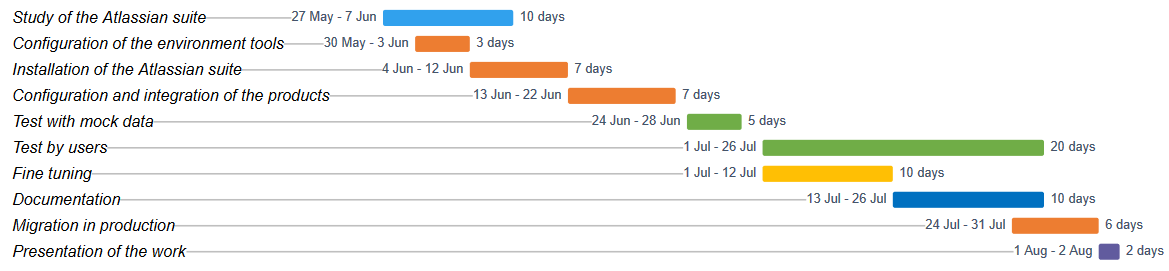
\includegraphics[width=22cm]{resources/work_plan_gantt}\\
		\caption{Gantt diagram contained in the ``\textit{Piano di Lavoro}'' document}
	\end{figure}
	\vspace*{\fill}
\end{landscape}
\newpage
\begin{landscape}
	\vspace*{\fill}
	\section{GANTT 2}
	\label{gantt_2}
	\begin{figure}[H]
		\centering
		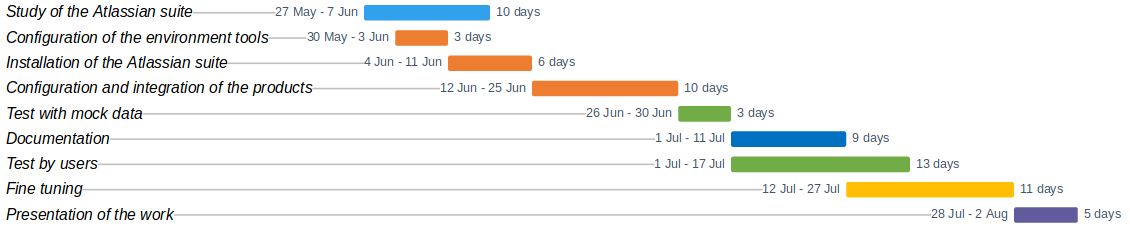
\includegraphics[width=22cm]{resources/revised_gantt}\\
		\caption{Gantt diagram contained in the ``\textit{Piano di Lavoro}'' document}
	\end{figure}
	\vspace*{\fill}
\end{landscape}